\documentclass[10pt,a4paper]{article}
\usepackage[a4paper, total={6in, 8in}]{geometry}
\usepackage{graphicx}


\begin{document}

\section{Task}

\subsection{Comparison of 1D and 2D decomposition}

\textbf{Describe the advantages/disadvantages of a two-dimensional decomposition (compared to a one-dimensional decomposition).}\\

At first glance, it seems to be an advantage of the 1D decomposition that only two neighbours have to be sent to, which 
means less work than sending to all four neighbours as in the 2D case. However, if you look at the actual data that is going 
to be sent and the time it takes, the 2D decomposition hase actually an advantage. A good parameter is the speedup, 
which is calculated by dividing the runtime $T_s$ by the parallel runtime $T_p$. $S = \frac{T_s}{T_p}$, this indicates 
how much the runtime changes by including more processes. Overall, it can be said that the scaling behaviour 
between 1D decomposition and 2D decomposition is significantly different, as the intersection of the 2D subdomains is 
smaller than in the 1D case. However, this does not have a significant effect on the speed-up when the number of CPU 
cores is small, but it does when the number is large. \\


To illustrate this, we can consider an example: We take a domain with a resolution of 250 and calculate 100 time steps. 
We describe $t_s$ as the time needed to calculate one iteration for one node and $t_p$ as the time needed to communicate 
with other cells and assume that both take one time unit. \\
\\
\begin{center}
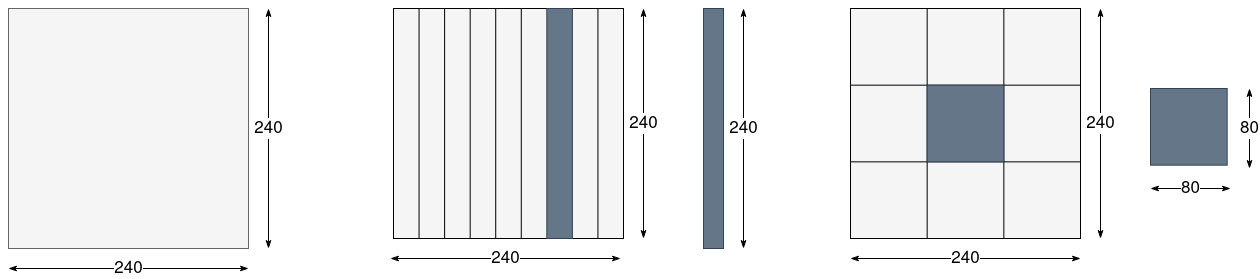
\includegraphics[width=14.5cm]{Task.png}
\end{center}

In the figure above, an area with a resolution of 240 is shown, the entire domain can be seen on the left. If a 1D 
decomposition were chosen, the sub-areas would look like the blue rectangle in the middle, with the cutting surface 
to be communicated being 2x240 = 480. The 2D decomposition is shown on the right. Here the edge of the subarea is 
4x80 = 320. \\

\begin{table}[h]
    \centering
    \begin{tabular}{l|l|l}
    \textbf{MIP processes} & \textbf{1D Speedup} & \textbf{2D Speedup} \\ \hline
    5                      & 4.8             & 4.97            \\ \hline
    25                     & 20.83           & 24.38           \\ \hline
    125                    & 62.5            & 110.96          \\ \hline
    250                    & 83.33           & 199.53          \\
    \end{tabular}
\end{table}

It can be seen from the table that the speedup scales much better with resolution in 2D decomposition, as the 
intersection of the domains remains the same in 1D at any resolution, but becomes smaller in 2D as the resolution 
increases. \\

Reference : https://alexander.vondrous.de/?p=7

\newpage
\subsection{Effect of decomposition on numercal solution}

\textbf{Discuss if the decomposition of the domain changes the order of computations performed during a single Jacobi 
iteration -  i.e., if you expect a numerically identical result after each iteration, or not.} \\

Since the decomposition now divides the area into smaller sub-areas, but does not change the actual values. Also, 
in our code, the boundaries of the subdomains are updated with the neighbouring values at each iteration. We expect 
that the result after each iteration will not be numerically different from the calculation without subdomains, to 
machine precision. If the ghost values were updated less frequently, we expect the error to increase. \\

\subsection{Depth of ghost layer}

\textbf{A generalization of the ghost layer approach would be to set the width of the ghost 
layer that is exchanged as a parameter W of the decomposition. This allows to perform W independent 
iterations before a communication of the ghost layers has to happen. Comment in which situation 
(w.r.t the available bandwidth or latency between MPI-processes) multiple independent iterations are 
potentially advantageous.} \\


In the approach of a ghost layer with a depth of one, one would have to update the boundaries of the sub-areas at 
each step and therefore send many messages with a small size. This is a large communication overhead. Generalising 
this approach, as described in the question, to a ghost layer with a width of W fixes this, but the number of ghost 
layers also corresponds to the accuracy of the numerical methods.\\

The idea behind this generalisation of the ghost layers is the increase in message volume with each update and 
correspondingly less frequent updating in general. This means with W = 6, the ghost layers only need to be updated 
once every five time steps, with six layers being exchanged at once. So with less frequent updates, smaller messages 
are combined into larger messages, allowing for higher communication bandwidth and lower communication latency. \\ 

This can be advantageous if the available bandwidth allows it. Since we are working with the IUE cluster, a bandwidth 
of 10Gbit/s is available. Even when reducing latency is the main goal, changing the width of the ghost layers can be 
a good approach. One disadvantage of a larger W is that this method requires more memory and computation than the 
traditional method, but this is a small difference compared to the total memory required. \\ 
 
Reference: DOI: 10.1109/SC.2001.10042 \\

\newpage
\subsection{Exchange with diagional neighbors}

\textbf{Assume a ghost layer with width W=1 (this is what you will later implement) 
and discuss if a data exchange between parts of the domain which are "diagonal neighbors" is 
required assuming a "5-point star-shaped stencil".} \\

Since we work with a "5-point star template", the diagonal elements are never needed for an iteration. Only the 
direct neighbours in the direction of north, south, west, east are needed. Furthermore, if the communication with 
the ghost layers involves all elements in a row/column, as implied in the task description and in the figure below, 
it is possible to exchange data with the "diagonal neighbours" in two steps as well. This is illustrated in the 
following figure. \\


\begin{center}
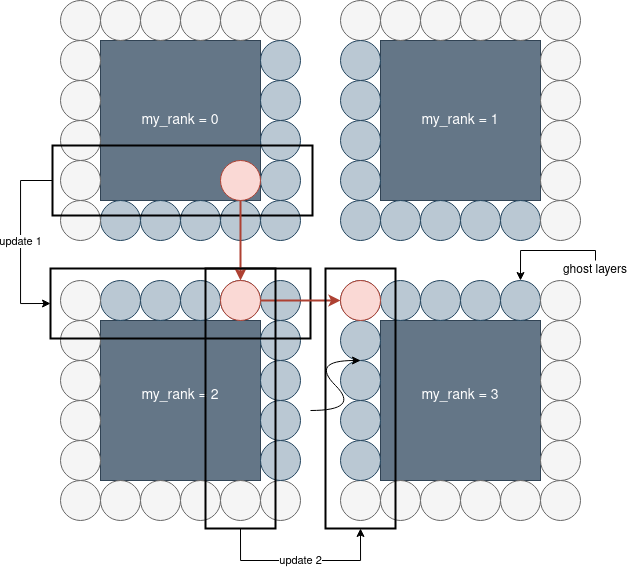
\includegraphics[width=7cm]{Diagonal.png}
\end{center}

\subsection{IUE-cluster}
\textbf{How big is the sum of all L2 caches for 2 nodes of the IUE-cluster }\\


Looking at the statistics of the IUE cluster, there are two types of computer nodes available, 10x normal 
computer nodes and 2x fat computer nodes. Both types are equipped with 2x INTEL Xeon Gold 6248, 2.5GHz, 20C/40T, 
as described on the official website. [1] So each processor has an L2 cache of 16MB [2], giving a total of 64MB 
for 2 nodes and 2 INTEL. \\


Reference:
\begin{enumerate}
    \item [1] https://www.iue.tuwien.ac.at/research/computing-infrastructure/
    \item [2] https://www.cpubenchmark.net
\end{enumerate}



\end{document}
